\documentclass{../../zirkelblatt}

\usepackage{geometry}
\geometry{tmargin=0.5cm,bmargin=0.5cm,lmargin=1cm,rmargin=1cm}

\pagestyle{empty}

\begin{document}

\makeatletter
\newcommand*{\shifttext}[2]{%
  \settowidth{\@tempdima}{#2}%
  \makebox[\@tempdima]{\hspace*{#1}#2}%
}
\makeatother

\newcommand{\vorderseite}{
  \begin{minipage}[t][4cm][t]{7.6cm}
    \begin{center}
      \textsf{The constant~$\tau$, a transcendental number}
      \vspace{0.6em}
      \tiny

      \makebox[0pt]{\shifttext{-6pt}{6,}}%
      283 185 3071 795 864 7692 528 676 6559 005 768 3943 387 987 5021 

      164 194 9889 184 615 6328 125 724 1799 725 606 9650 684 234 1359 

      642 961 7302 656 461 3294 187 689 2191 011 644 6345 071 881 6256 

      962 234 9005 682 054 0387 704 221 1119 289 245 8979 098 607 6392 

      885 762 1951 331 866 8922 569 512 9646 757 356 6330 542 403 8182

      912 971 3384 692 069 7220 908 653 2964 267 872 1452 049 828 2547

      449 174 0132 126 311 7634 976 304 1841 925 658 5081 834 307 2873

      578 518 0720 022 661 0610 976 409 3304 276 829 3903 883 023 2188

      661 145 4073 151 918 3906 184 372 2347 638 652 2358 621 023 7096

      148 924 7599 254 991 3470 377 150 5449 782 455 8763 660 238 9825
    \end{center}

    \vfill
    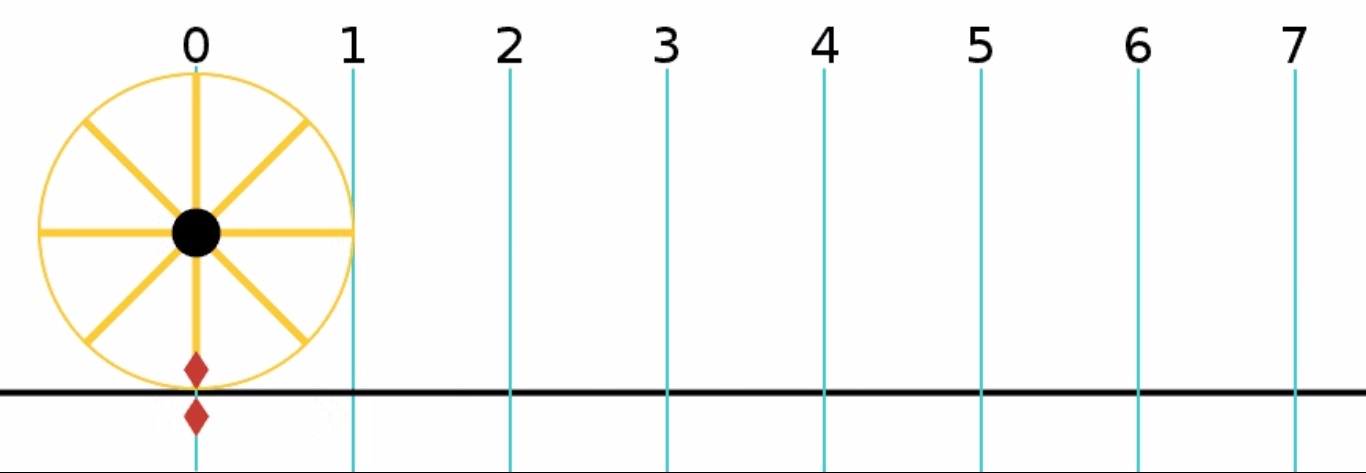
\includegraphics[scale=0.170]{tau-1}\hfill%
    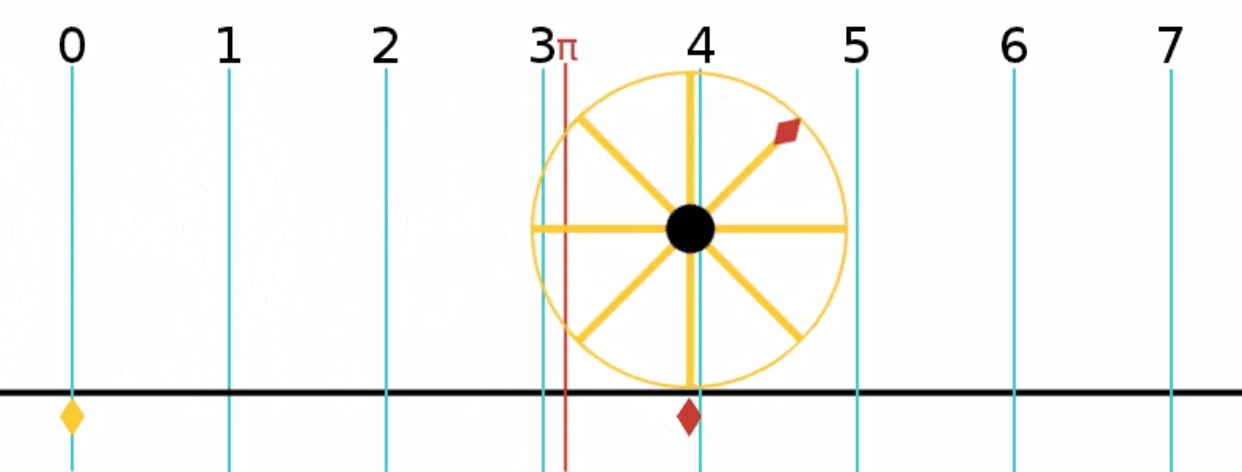
\includegraphics[scale=0.170]{tau-2}\hfill%
    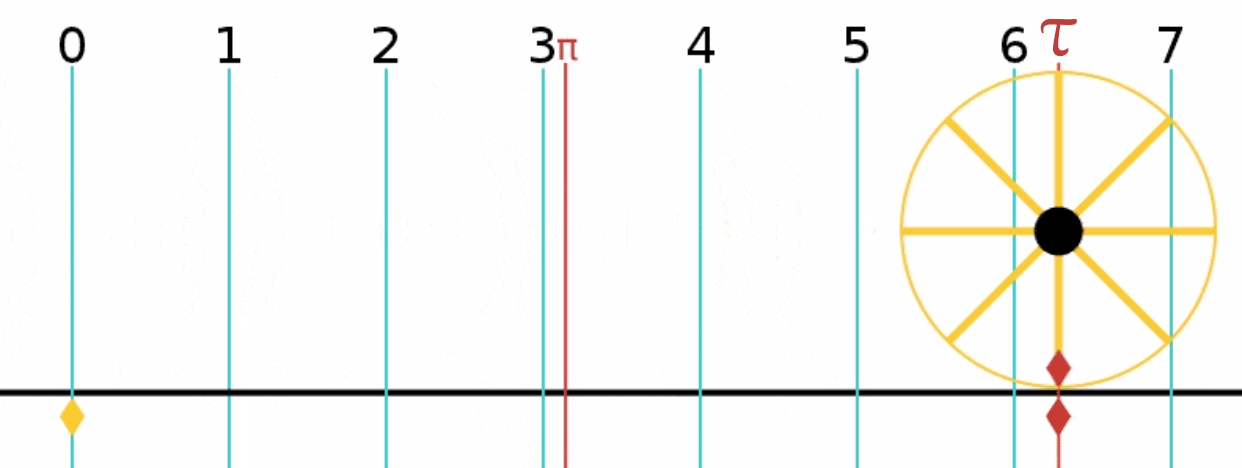
\includegraphics[scale=0.170]{tau-3}
  \end{minipage}
}

\newcommand{\rueckseite}{
  \begin{minipage}[t][4cm][t]{7.6cm}
    \phantom{A}
    \vspace{-0.3em}
    \tiny

    Fans celebrate the international \textbf{$\boldsymbol{\tau}$ day} on June 28th.
    They think that~$\tau$ is twice as good as~$\pi = \tau/2$,
    because many formulas don't actually involve~$\pi$, but~$2\pi$ as a unit;
    and interpreted as radians,~$\tau$ corresponds to the full circle
    while~$\pi$ only corresponds to the semi circle.
    The \textbf{continued fraction expansion} yields~$19:3$ as an
    \textbf{approximation} for~$\tau$.
    %Das Symbol ist ein Buchstabe aus dem griechischen Alphabet und wird
    %\textbf{Tau} ausgesprochen.
    Its decimal expansion contains a sequence of~\textbf{seven nines} starting
    at position~761. The \textbf{circumference} of a circle with radius~$r$ is
    $\tau r$. Its
    \textbf{area} is~$\frac{1}{2} \tau r^2$.
    The number~$\tau$ is \textbf{irrational}, hence cannot be written as a
    fraction of integers. It is even~\textbf{transcendental}, hence not a
    solution of any polynomial equation.
    \textbf{Open question:} Do the ten digits occur equally often in the
    decimal expansion of~$\tau$?
    \scalebox{0.7}{\begin{minipage}{1.42\textwidth}
    \vspace{-1.3em}
    \begin{align*}
      1 - \frac{1}{3} + \frac{1}{5} - \frac{1}{7} + \frac{1}{9} - \dots &= \frac{\tau}{8} &
      1 &= e^{i \tau} &
      \tau &= 6 + \frac{1}{3 + \frac{1}{1 + \frac{1}{1 + \cdots}}} \\
      \frac21 \cdot \frac23 \cdot \frac43 \cdot \frac45 \cdot \frac65 \cdot
      \frac67 \cdot \frac87 \cdot \frac89 \cdot \dots &= \frac{\tau}{4} &
      \chi(M) &= \frac{1}{\tau} \int_M K \,dA &
      f(z) &= \frac{1}{\tau i} \oint \frac{f(\zeta)}{\zeta - z} \,d\zeta
    \end{align*}\end{minipage}}
  \end{minipage}
}

\vorderseite\hfill\vorderseite
\vfill
\vorderseite\hfill\vorderseite
\vfill
\vorderseite\hfill\vorderseite
\vfill
\vorderseite\hfill\vorderseite
\vfill
\vorderseite\hfill\vorderseite

\newpage

\sffamily
%\fontfamily{kurier}\selectfont

\rueckseite\hfill\rueckseite
\vfill
\rueckseite\hfill\rueckseite
\vfill
\rueckseite\hfill\rueckseite
\vfill
\rueckseite\hfill\rueckseite
\vfill
\rueckseite\hfill\rueckseite

\end{document}

983 367 3362 440 656 6430 860 213 9494 639 522 4737 190 702 1798
609 437 0277 053 921 7176 293 176 7523 846 748 1846 766 940 5132
000 568 1271 452 635 6082 778 577 1342 757 789 6091 736 371 7872
146 844 0901 224 953 4301 465 495 8537 105 079 2279 689 258 9235
420 199 5611 212 902 1960 864 034 4181 598 136 2977 477 130 9960
518 707 2113 499 999 9837 297 804 9951 059 731 7328 160 963 1859
502 445 9455 346 908 3026 425 223 0825 334 468 5035 261 931 1881
710 100 0313 783 875 2886 587 533 2083 814 206 1717 766 914 7303
598 253 4904 287 554 6873 115 956 2863 882 353 7875 937 519 5778
185 778 0532 171 226 8066 130 019 2787 661 119 5909 216 420 1989
380 952 5720 106 548 5863 278 865 9361 533 818 2796 823 030 1952
035 301 8529 689 957 7362 259 941 3891 249 721 7752 834 791 3151
557 485 7242 454 150 6959 508 295 3311 686 172 7855 889 075 0983
817 546 3746 493 931 9255 060 400 9277 016 711 3900 984 882 4012
858 361 6035 637 076 6010 471 018 1942 955 596 1989 467 678 3744
944 825 5379 774 726 8471 040 475 3464 620 804 6684 259 069 4912
933 136 7702 898 915 2104 752
